\chapter{Motivation}\label{blabli}
Code: \url{https://github.com/NeverL8/ADL/tree/main/B07}
\vspace{0.75cm}\newline
Previously we have used GANs in order to generate samples, i.e. digits, based on the MNIST dataset. The adversarial approach of GANs with
a discriminator trying to identify fake images has some critical downsides. Convergence is not guaranteed, there is no inherent evalution metric
for sample quality and the generator can fall into mode collapse (only generating a few kinds of samples).
Diffusion models on the other hand do not require adversarial training, are parallelizable and scalable and promise convergence in a stable manner.
They are based on gradual Markov chain noise generation in a forward process and are trained to predict the
added noise in a backward process (denoising).
Conclusively, the computational cost of diffusion models is extremely high.
In this exercise we will try to generate MNIST digits using Phil Wang's "denoising-diffusion pytorch"\cite{lucidrains_denoising_diffusion_pytorch}
library, which is a more complex application than generating numbers
resembling a bimodal distribution of two gaussians like in last week's exercise.
\chapter{Code architecture}
A typical structure of image generation diffusion models is an U-net, which
is also the architecture we will use here. It provides precise spatial reconstruction as well as global feature abstraction.
The following network definition (as given in the template) is utilized:
\begin{minted}{python}
DIM = 32
DIM_MULTS = (1, 2, 5)
model = Unet(
    dim = DIM,
    dim_mults = DIM_MULTS,
    flash_attn = False,
    channels = 1
)
\end{minted}
The following hyperparameters have been used.
\begin{minted}{python}
LEARNING_RATE = 4e-4
BATCH_SIZE = 128  # Batch size
N_EPOCHS = 100
IMAGE_SIZE = 28
TIME_STEPS = 1000
SAMPLING_TIMESTEPS = 250
\end{minted}
The remaining code is trivial and can be found using the link given in \autoref{blabli}.
\chapter{Results and observations}
First and foremost, the most striking observation is that computation
takes quite long despite using a T4 GPU ($\sim\qty{2}{\minute\per\text{epoch}}$).
The loss curves in \autoref{loss} show fast convergence within the first roughly 20 epochs and a much slower but steady decrease in loss afterwards.
\begin{figure}[h]
    \centering
    
\includegraphics[width=0.7\textwidth]{../data/fullLossCurve.png}
    \caption{Loss curves.}\label{loss}
\end{figure}
\autoref{stuff} depicts images generated at various epochs of training.
As the loss curves suggest, most of the improvements occur in the early epochs.
The digits of the fully trained network in \autoref{comparison} however still contain a few not clearly recognizable samples.

\begin{longtable}{>{\centering\arraybackslash}m{0.48\textwidth}
                  >{\centering\arraybackslash}m{0.48\textwidth}}
\textbf{$n=5$} & \textbf{$n=10$} \\

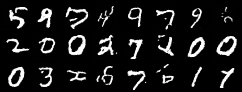
\includegraphics[width=0.95\linewidth]{../data/new_generated_digits_epoch_5.png} &
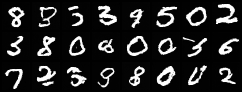
\includegraphics[width=0.95\linewidth]{../data/new_generated_digits_epoch_10.png} \\[1em]

\textbf{$n=20$} & \textbf{$n=30$} \\

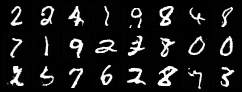
\includegraphics[width=0.95\linewidth]{../data/new_generated_digits_epoch_20.png} &
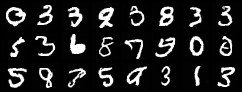
\includegraphics[width=0.95\linewidth]{../data/new_generated_digits_epoch_30.png} \\[1em]

\textbf{$n=40$} & \textbf{$n=50$} \\

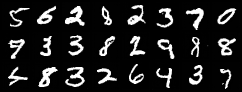
\includegraphics[width=0.95\linewidth]{../data/new_generated_digits_epoch_40.png} &
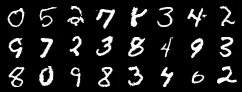
\includegraphics[width=0.95\linewidth]{../data/new_generated_digits_epoch_50.png} \\[1em]

\textbf{$n=60$} & \textbf{$n=70$} \\

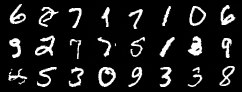
\includegraphics[width=0.95\linewidth]{../data/new_generated_digits_epoch_60.png} &
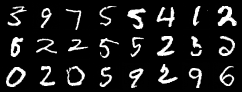
\includegraphics[width=0.95\linewidth]{../data/new_generated_digits_epoch_70.png} \\[1em]

\textbf{$n=80$} & \textbf{$n=90$} \\

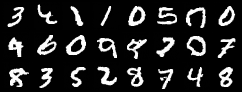
\includegraphics[width=0.95\linewidth]{../data/new_generated_digits_epoch_80.png} &
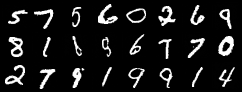
\includegraphics[width=0.95\linewidth]{../data/new_generated_digits_epoch_90.png}
\end{longtable}
\captionof{figure}{Digits generated after $n$ training epochs.}
\label{stuff}

\autoref{comparison} compares 32 digits generated with the fully trained DDPM model (after 100 epochs) to the GAN-generated digits from two exercises ago.
\begin{figure}[htbp]
    \centering

    \begin{subfigure}{0.6\textwidth}
        \centering
        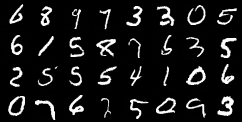
\includegraphics[width=\linewidth]{../data/new_generated_digits_epoch_100.png}
        \caption{Generated digits for fully trained DDPM (Epoch 100).}
    \end{subfigure}

    \vspace{1em}

    \begin{subfigure}{0.6\textwidth}
        \centering
        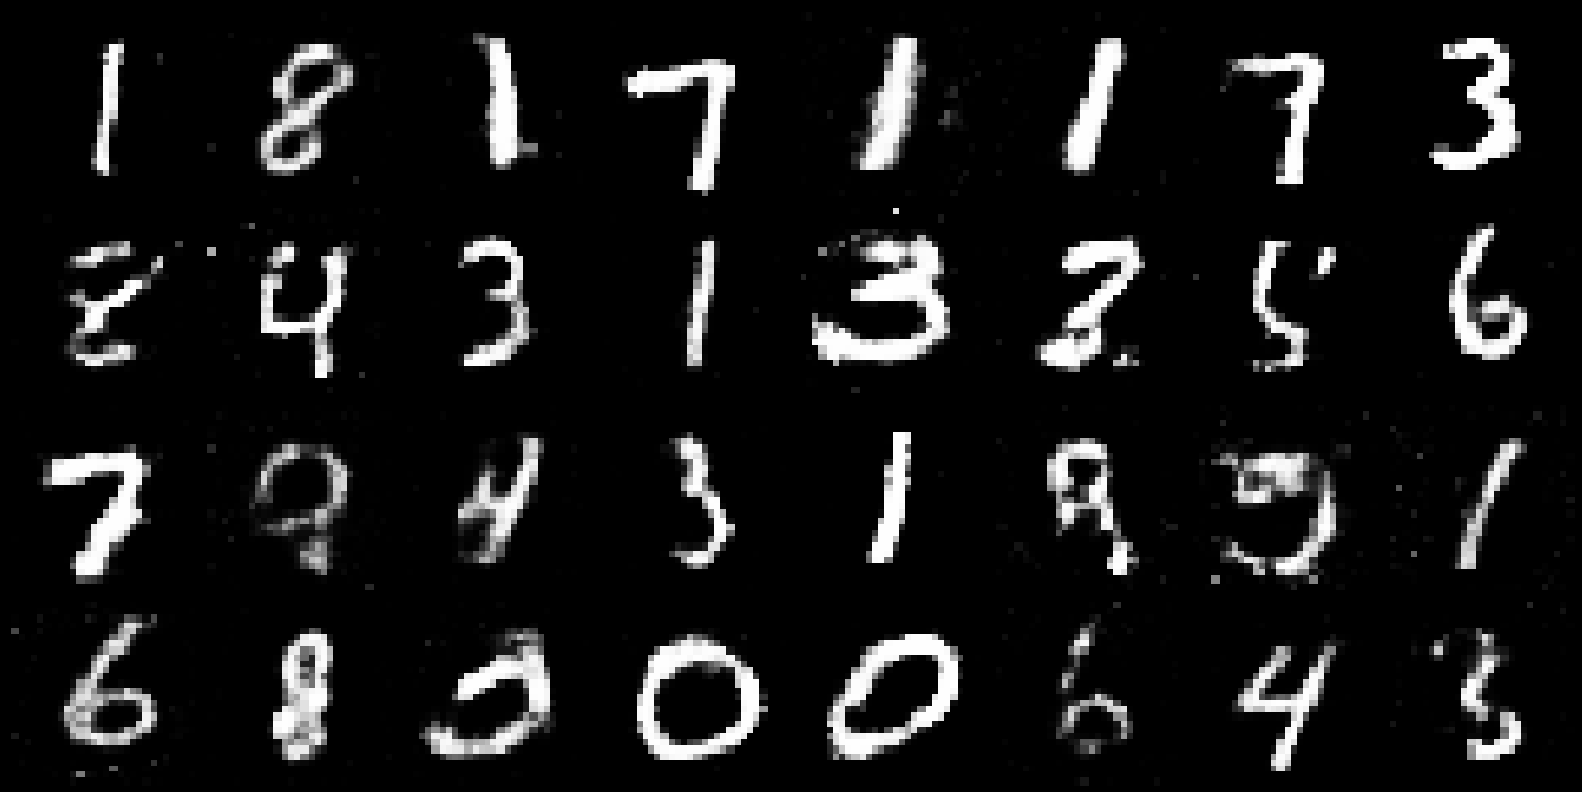
\includegraphics[width=\linewidth]{../GAN_lastEpoch.png}
        \caption{Generated digits for fully trained GAN.}
    \end{subfigure}
\caption{Comparison of GAN and diffusion generated digits.}\label{comparison}

\end{figure}


\chapter{Conclusion}
Contrary to the GAN-generated images, the diffusion-generated images
show fewer artifacts (individual white pixels) and greyish areas within the digits.
The logic that the centres of the lines are bright, the background is black and the edges
fade between both completely applies to the diffusion-generated samples. 
One can also observe variable line thickness of different samples. 
Some samples are still not completely distinct even after 100 epochs.
It is unclear whether further training could improve the remaining samples as one cannot certainly tell from \autoref{loss} whether the loss decrease has already saturated.
One could likely also improve results by training for each label (i.e. digit) seperately or optimizing network hyperparameters (which I do not want to waste time on).